%!TEX root = ../proposal-presentation.tex

\begin{frame}[t] \frametitle{1. Test Data}

	\textbf{Aim: to have appropriate data for development}

	\vfill

	\onslide<+->
	{

	\begin{columns}[c]

	\column{0.5\linewidth}
		For initial development:

		\begin{itemize}\itemsep10pt
			\item Publicly available RGB-D datasets
			\item cf. \cite{firman2016}
		\end{itemize}

	\column{0.5\linewidth}
		\begin{figure}
		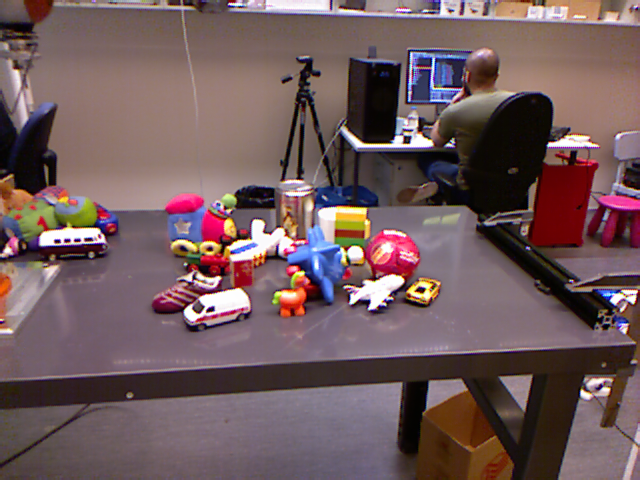
\includegraphics[width=\linewidth]{src/toydataset.png}
		\caption{Toy dataset \cite{ikkala2016}}
		\end{figure}

	\end{columns}

	}

	\vfill

	\onslide<+->
	{

	For embodied testing:

	\begin{itemize}\itemsep10pt
		\item Create at least one physical scene
	\end{itemize}

	}

	\vfill

\end{frame}


\begin{frame}[t] \frametitle{2. Object Discovery on Single Images}

	\textbf{Aim: to be able to accurately detect objects in a static image}

	\vfill

	\begin{itemize}
		\item Saliency-based system \cite{garcia2013computational}
	\end{itemize}

	\vfill

	\centering

	\begin{figure}
	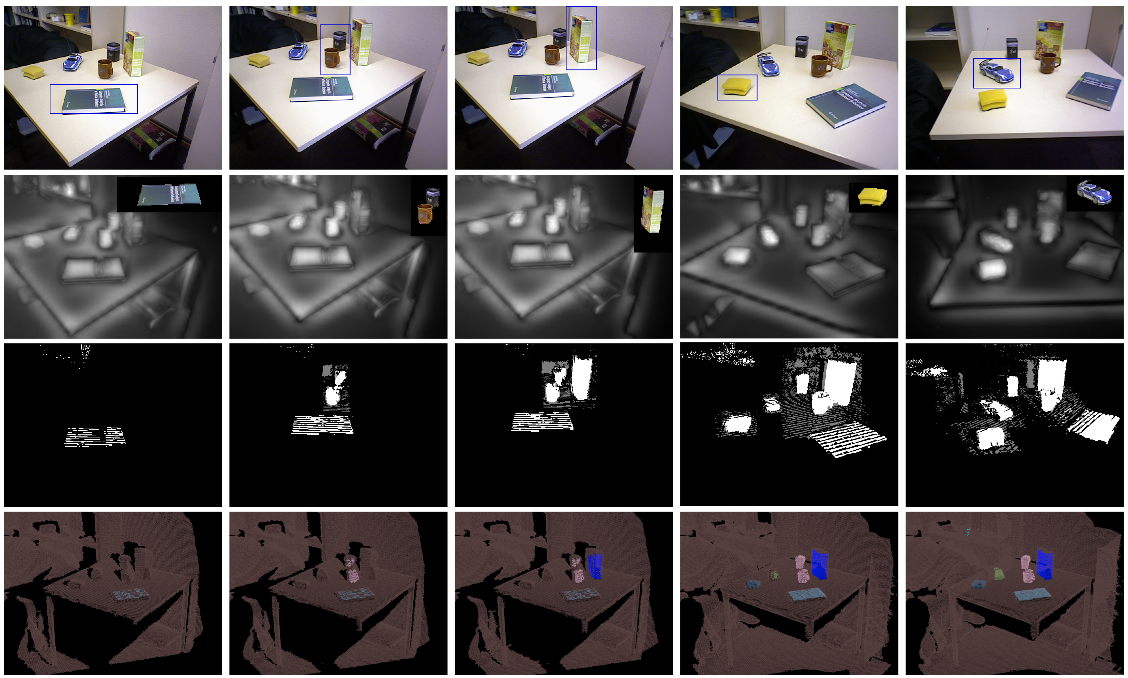
\includegraphics[width=0.8\linewidth]{src/garcia2013fig4.png}
	\end{figure}

\end{frame}


\begin{frame}[t] \frametitle{3. Determining the Next Best View}

	\textbf{Aim: to be able to calculate the optimal viewing angle}

	\onslide<+->
	{

	Possible implementations:

	\begin{itemize}
		\item Subsumption architecture \cite{brooks1986robust}
		\item Information gain \cite{surmann2003autonomous}
		\item POMDPs \cite{lauri2015planning}
	\end{itemize}

	}

	\onslide<+->
	{

	Possible baselines:

	\begin{itemize}
		\item No movement
		\item Randomised movements
		\item Hardcoded path
	\end{itemize}

	}

	\vfill

	\onslide<+->
	{
	\textbf{Question:} update while the robot is moving?
	}

\end{frame}


\begin{frame}[t] \frametitle{4. Fusing Multiple Views}

	\textbf{Aim: to be able to create a 3D model from multiple 2D images}

	\medskip

	\begin{itemize}

		% \item Solve SLAM problem

		% \begin{itemize}\itemsep10pt
		% 	\item FastSLAM
		% 	\item RatSLAM
		% 	\item \ldots
		% \end{itemize}

		% \medskip

		\item KinectFusion
		\medskip
		\begin{itemize}
			\item Implemented in PCL ("KinFu")
		\end{itemize}

		% \item Fuse 2D images to 3D model

		% \begin{itemize}\itemsep10pt
		% 	\item KinectFusion
		% \end{itemize}

	\end{itemize}

	\vfill

	\centering
	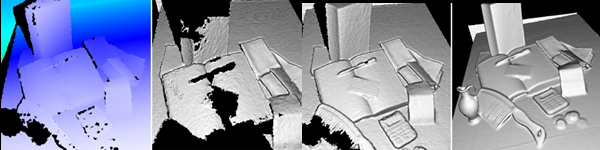
\includegraphics[width=.8\linewidth]{src/kinectfusion.png}



\end{frame}


\begin{frame}[t] \frametitle{5. Moving the Robot}

	\textbf{Aim: to be able to move the robot to a specific point}

	\bigskip

	\begin{itemize}\itemsep16pt
		\item ROS navigation stack
		\medskip
		\begin{itemize}\itemsep10pt
			\item \texttt{MoveBaseAction}
			\item \texttt{actionlib}
		\end{itemize}
	\end{itemize}

	\vfill

	\flushright
	
\includegraphics[width=0.8\linewidth]{src/ros.png}

	\vfill

\end{frame}


\begin{frame}[t] \frametitle{6. System Evaluation}

	\textbf{Aim: optimisation and comparison}

	\vfill

	\begin{itemize}\itemsep16pt
		\item Find optimal parameters
		\item Compare next best view approaches
		\medskip
		\begin{itemize}\itemsep10pt
			\item Random movements
			\item Hardcoded path
			\item Previously mentioned approaches
		\end{itemize}
	\end{itemize}

	\vfill

\end{frame}
